% Options for packages loaded elsewhere
\PassOptionsToPackage{unicode}{hyperref}
\PassOptionsToPackage{hyphens}{url}
\PassOptionsToPackage{dvipsnames,svgnames,x11names}{xcolor}
\documentclass[
  12pt,
]{scrreprt}
\usepackage{xcolor}
\usepackage[margin=1in]{geometry}
\usepackage{amsmath,amssymb}
\setcounter{secnumdepth}{5}
\usepackage{iftex}
\ifPDFTeX
  \usepackage[T1]{fontenc}
  \usepackage[utf8]{inputenc}
  \usepackage{textcomp} % provide euro and other symbols
\else % if luatex or xetex
  \usepackage{unicode-math} % this also loads fontspec
  \defaultfontfeatures{Scale=MatchLowercase}
  \defaultfontfeatures[\rmfamily]{Ligatures=TeX,Scale=1}
\fi
\usepackage{lmodern}
\ifPDFTeX\else
  % xetex/luatex font selection
  \setmainfont[]{Garamond}
  \setsansfont[]{Gotham-Book.otf}
  \setmonofont[]{Courier New}
\fi
% Use upquote if available, for straight quotes in verbatim environments
\IfFileExists{upquote.sty}{\usepackage{upquote}}{}
\IfFileExists{microtype.sty}{% use microtype if available
  \usepackage[]{microtype}
  \UseMicrotypeSet[protrusion]{basicmath} % disable protrusion for tt fonts
}{}
\makeatletter
\@ifundefined{KOMAClassName}{% if non-KOMA class
  \IfFileExists{parskip.sty}{%
    \usepackage{parskip}
  }{% else
    \setlength{\parindent}{0pt}
    \setlength{\parskip}{6pt plus 2pt minus 1pt}}
}{% if KOMA class
  \KOMAoptions{parskip=half}}
\makeatother
\usepackage{color}
\usepackage{fancyvrb}
\newcommand{\VerbBar}{|}
\newcommand{\VERB}{\Verb[commandchars=\\\{\}]}
\DefineVerbatimEnvironment{Highlighting}{Verbatim}{commandchars=\\\{\}}
% Add ',fontsize=\small' for more characters per line
\usepackage{framed}
\definecolor{shadecolor}{RGB}{248,248,248}
\newenvironment{Shaded}{\begin{snugshade}}{\end{snugshade}}
\newcommand{\AlertTok}[1]{\textcolor[rgb]{0.94,0.16,0.16}{#1}}
\newcommand{\AnnotationTok}[1]{\textcolor[rgb]{0.56,0.35,0.01}{\textbf{\textit{#1}}}}
\newcommand{\AttributeTok}[1]{\textcolor[rgb]{0.13,0.29,0.53}{#1}}
\newcommand{\BaseNTok}[1]{\textcolor[rgb]{0.00,0.00,0.81}{#1}}
\newcommand{\BuiltInTok}[1]{#1}
\newcommand{\CharTok}[1]{\textcolor[rgb]{0.31,0.60,0.02}{#1}}
\newcommand{\CommentTok}[1]{\textcolor[rgb]{0.56,0.35,0.01}{\textit{#1}}}
\newcommand{\CommentVarTok}[1]{\textcolor[rgb]{0.56,0.35,0.01}{\textbf{\textit{#1}}}}
\newcommand{\ConstantTok}[1]{\textcolor[rgb]{0.56,0.35,0.01}{#1}}
\newcommand{\ControlFlowTok}[1]{\textcolor[rgb]{0.13,0.29,0.53}{\textbf{#1}}}
\newcommand{\DataTypeTok}[1]{\textcolor[rgb]{0.13,0.29,0.53}{#1}}
\newcommand{\DecValTok}[1]{\textcolor[rgb]{0.00,0.00,0.81}{#1}}
\newcommand{\DocumentationTok}[1]{\textcolor[rgb]{0.56,0.35,0.01}{\textbf{\textit{#1}}}}
\newcommand{\ErrorTok}[1]{\textcolor[rgb]{0.64,0.00,0.00}{\textbf{#1}}}
\newcommand{\ExtensionTok}[1]{#1}
\newcommand{\FloatTok}[1]{\textcolor[rgb]{0.00,0.00,0.81}{#1}}
\newcommand{\FunctionTok}[1]{\textcolor[rgb]{0.13,0.29,0.53}{\textbf{#1}}}
\newcommand{\ImportTok}[1]{#1}
\newcommand{\InformationTok}[1]{\textcolor[rgb]{0.56,0.35,0.01}{\textbf{\textit{#1}}}}
\newcommand{\KeywordTok}[1]{\textcolor[rgb]{0.13,0.29,0.53}{\textbf{#1}}}
\newcommand{\NormalTok}[1]{#1}
\newcommand{\OperatorTok}[1]{\textcolor[rgb]{0.81,0.36,0.00}{\textbf{#1}}}
\newcommand{\OtherTok}[1]{\textcolor[rgb]{0.56,0.35,0.01}{#1}}
\newcommand{\PreprocessorTok}[1]{\textcolor[rgb]{0.56,0.35,0.01}{\textit{#1}}}
\newcommand{\RegionMarkerTok}[1]{#1}
\newcommand{\SpecialCharTok}[1]{\textcolor[rgb]{0.81,0.36,0.00}{\textbf{#1}}}
\newcommand{\SpecialStringTok}[1]{\textcolor[rgb]{0.31,0.60,0.02}{#1}}
\newcommand{\StringTok}[1]{\textcolor[rgb]{0.31,0.60,0.02}{#1}}
\newcommand{\VariableTok}[1]{\textcolor[rgb]{0.00,0.00,0.00}{#1}}
\newcommand{\VerbatimStringTok}[1]{\textcolor[rgb]{0.31,0.60,0.02}{#1}}
\newcommand{\WarningTok}[1]{\textcolor[rgb]{0.56,0.35,0.01}{\textbf{\textit{#1}}}}
\usepackage{graphicx}
\makeatletter
\newsavebox\pandoc@box
\newcommand*\pandocbounded[1]{% scales image to fit in text height/width
  \sbox\pandoc@box{#1}%
  \Gscale@div\@tempa{\textheight}{\dimexpr\ht\pandoc@box+\dp\pandoc@box\relax}%
  \Gscale@div\@tempb{\linewidth}{\wd\pandoc@box}%
  \ifdim\@tempb\p@<\@tempa\p@\let\@tempa\@tempb\fi% select the smaller of both
  \ifdim\@tempa\p@<\p@\scalebox{\@tempa}{\usebox\pandoc@box}%
  \else\usebox{\pandoc@box}%
  \fi%
}
% Set default figure placement to htbp
\def\fps@figure{htbp}
\makeatother
\setlength{\emergencystretch}{3em} % prevent overfull lines
\providecommand{\tightlist}{%
  \setlength{\itemsep}{0pt}\setlength{\parskip}{0pt}}
\usepackage[round,authoryear]{natbib}
\bibliographystyle{apalike}
% header.tex
\usepackage{graphicx}
\usepackage{titling}
\usepackage{fancyhdr}
\usepackage{fontspec}   % For loading fonts
\usepackage{xcolor}     % For color definitions
\usepackage{mdframed}
\usepackage{tocloft}    % For customizing the TOC

% Define the Boise State Blue color
\definecolor{boisestateblue}{HTML}{0033A0}

% Load Gotham fonts
\newfontface\gothamblack{Gotham-Black.otf}[Path=../Document_fonts/]
\newfontface\gothambold{Gotham-Bold_0.otf}[Path=../Document_fonts/]
\newfontface\gothambolditalic{Gotham-BoldItalic.otf}[Path=../Document_fonts/]
\newfontface\gothambook{Gotham-Book.otf}[Path=../Document_fonts/]
\newfontface\gothammedium{Gotham-Medium.otf}[Path=../Document_fonts/]

% Set the document's main font to Garamond
\setmainfont{Garamond}
% Set the sans-serif font (used for headings) to Gotham Book
\setsansfont{Gotham-Book.otf}[Path=../Document_fonts/]
% Set the monospace font to Garamond
\setmonofont{Garamond}

% -----------------------------------------------------------------------------
% Style the Table of Contents using tocloft + Gotham
% -----------------------------------------------------------------------------
\renewcommand{\cfttoctitlefont}{\Huge \sffamily \bfseries \color{boisestateblue}}
\renewcommand{\cftsecfont}{\normalfont\sffamily}
\renewcommand{\cftsecpagefont}{\normalfont\sffamily}
\renewcommand{\cftsubsecfont}{\normalfont\sffamily}
\renewcommand{\cftsubsecpagefont}{\normalfont\sffamily}
\renewcommand{\cftsubsubsecfont}{\normalfont\sffamily}
\renewcommand{\cftsubsubsecpagefont}{\normalfont\sffamily}

\cftsetindents{section}{0em}{2.5em}
\cftsetindents{subsection}{1.5em}{3.5em}
\cftsetindents{subsubsection}{3em}{4.5em}

% -----------------------------------------------------------------------------
% Define the custom title page style with the logo
% -----------------------------------------------------------------------------
\fancypagestyle{titlepage}{
  \fancyhf{} % Clear all headers/footers
  \fancyfoot[C]{
    \begin{minipage}{\textwidth}
      \centering
      \vspace{-3cm}
      
\includegraphics[width=0.4\textwidth]{../images/boisestate-primarylogo-1color-orange-rgb.png}
    \end{minipage}
  }
  \renewcommand{\headrulewidth}{0pt}
  \renewcommand{\footrulewidth}{0pt}
}

% -----------------------------------------------------------------------------
% Custom maketitle: No page number on cover
% -----------------------------------------------------------------------------
\renewcommand{\maketitle}{
  \thispagestyle{titlepage}  % style with no visible page number
  \begin{center}
    \vspace*{3cm}
    {\Huge\sffamily\bfseries\color{boisestateblue}\thetitle}\\[4cm]

    \vspace*{1cm}
    {\Large\sffamily\color{boisestateblue}\theauthor}\\[0.5cm]
    {\large\sffamily\color{boisestateblue}\thedate}
  \end{center}
  \clearpage
  \thispagestyle{empty}  % also no page # on next side
  %
  % Now we start real numbering in Arabic:
  \pagenumbering{arabic}
  \setcounter{page}{1}
}

% -----------------------------------------------------------------------------
% If you redefined \tableofcontents before, remove that code. Let R Markdown do it
% and it will appear as page 1 (the first counted page).
% -----------------------------------------------------------------------------

% -----------------------------------------------------------------------------
% Customize links
% -----------------------------------------------------------------------------
\usepackage{hyperref}
\hypersetup{
    colorlinks=true,
    linkcolor=boisestateblue,
    urlcolor=D64309,
    citecolor=green
}

% -----------------------------------------------------------------------------
% Customize chapter titles for scrreprt (optional)
% -----------------------------------------------------------------------------
\renewcommand{\chapterformat}{\thechapter.\ }

% -----------------------------------------------------------------------------
%  Guiding Questions custom styled text box using mdframed
% -----------------------------------------------------------------------------
\usepackage{mdframed}

% Define the style for the text box
\newmdenv[
    linewidth=0.5pt,              % Border thickness
    linecolor=black,              % Border color
    backgroundcolor=lightgray!20, % Light gray background
    innerleftmargin=1em,          % Padding inside the box (left)
    innerrightmargin=1em,         % Padding inside the box (right)
    innertopmargin=1em,           % Padding inside the box (top)
    innerbottommargin=1em,        % Padding inside the box (bottom)
    skipabove=1em,                % Space above the box
    skipbelow=1em,                % Space below the box
    nobreak=true                  % Prevents splitting across pages
]{customtextbox}
% -----------------------------------------------------------------------------
% Include bibliography in the TOC and number it
% -----------------------------------------------------------------------------
\AtBeginDocument{
  \renewcommand{\bibname}{References}
  \renewcommand{\refname}{References}
}
\usepackage{bookmark}
\IfFileExists{xurl.sty}{\usepackage{xurl}}{} % add URL line breaks if available
\urlstyle{same}
\hypersetup{
  pdftitle={Chapter 5},
  pdfauthor={Lorraine Gaudio},
  colorlinks=true,
  linkcolor={boisestateblue},
  filecolor={Maroon},
  citecolor={black},
  urlcolor={magenta},
  pdfcreator={LaTeX via pandoc}}

\title{Chapter 5}
\usepackage{etoolbox}
\makeatletter
\providecommand{\subtitle}[1]{% add subtitle to \maketitle
  \apptocmd{\@title}{\par {\large #1 \par}}{}{}
}
\makeatother
\subtitle{Help!}
\author{Lorraine Gaudio}
\date{Version April 21, 2026}

\begin{document}
\maketitle

{
\hypersetup{linkcolor=}
\setcounter{tocdepth}{1}
\tableofcontents
}
\chapter{Overview}\label{overview}

In this chapter, you'll learn how to turn your R Notebook into a
shareable HTML report that another person can read \textbf{without
opening RStudio}! You'll start by using Markdown to make your notebook
readable and navigable by adding a date in the YAML header and headings
that create an outline so your work looks like a structured report. Then
you'll generate an HTML version of the notebook and learn how to
recognize (and troubleshoot) common problems when the report fails to
build. Because modern researchers often use AI tools during debugging,
you'll also learn how to write well-structured Markdown prompts to ask
an LLM for targeted help without delegating your thinking. This matters
now because, moving forward, you will be evaluated on whether your
workflow is understandable and reproducible (CLO1), whether you can
diagnose problems when something breaks (CLO2), and whether you can
document responsible help-seeking and tool use as part of your process
(CLO3).

In Chapter Five you will learn how to:

\begin{itemize}
\item
  \#️⃣ Format your R Notebook using Markdown
\item
  📐 Structure prompts for Large Language Models (LLMs)
\end{itemize}

\chapter{R Notebook -\textgreater{} HTML
Report}\label{r-notebook---html-report}

🎯 Please open a new R Notebook and save it in your course folder named
\texttt{chapter5\_notes.Rmd}. Use this document to take notes and
practice the chapter content.

\begin{enumerate}
\def\labelenumi{\arabic{enumi}.}
\item
  Open RStudio → File → New File → R Notebook.
\item
  Save it in your course folder as: \texttt{chapter5\_notes.Rmd}.
\item
  In your YAML header at the top, make sure the title matches this
  chapter.
\end{enumerate}

\section{YAML Date Field}\label{yaml-date-field}

The YAML header is the metadata ``label'' for your notebook. It controls
document settings like title and output format. A basic YAML header
looks like this:

\begin{Shaded}
\begin{Highlighting}[]
\PreprocessorTok{{-}{-}{-}}
\FunctionTok{title}\KeywordTok{:}\AttributeTok{ }\StringTok{"Untitled"}
\FunctionTok{output}\KeywordTok{:}\AttributeTok{ html\_notebook}
\PreprocessorTok{{-}{-}{-}}
\end{Highlighting}
\end{Shaded}

To add a date to your notebook, edit the YAML header to include a
\texttt{date:} field.

Method A. \textbf{Hard Code}

Manually type the date you created the notebook. Include quotation marks
around the date.

\begin{Shaded}
\begin{Highlighting}[]
\PreprocessorTok{{-}{-}{-}}
\FunctionTok{title}\KeywordTok{:}\AttributeTok{ }\StringTok{"Chapter 5 Practice"}
\FunctionTok{date}\KeywordTok{:}\AttributeTok{ }\StringTok{"January 13, 2026"}
\FunctionTok{output}\KeywordTok{:}\AttributeTok{ html\_notebook}
\PreprocessorTok{{-}{-}{-}}
\end{Highlighting}
\end{Shaded}

Method B. \textbf{Dynamic Date}

Use R code to generate the current date automatically each time you knit
the document. The inline R expression `r Sys.Date()` retrieves the
current date from your computer's operating system. This follows the
syntax: backtick (`), then r, a space, Sys.Date(), and a closing
backtick (`). The backtick is located above the Tab key on most
keyboards.

\begin{Shaded}
\begin{Highlighting}[]
\PreprocessorTok{{-}{-}{-}}
\FunctionTok{title}\KeywordTok{:}\AttributeTok{ }\StringTok{"Chapter 5 Practice"}
\FunctionTok{date}\KeywordTok{:}\AttributeTok{ }\StringTok{"\textasciigrave{}r Sys.Date()\textasciigrave{}"}
\FunctionTok{output}\KeywordTok{:}\AttributeTok{ html\_notebook}
\PreprocessorTok{{-}{-}{-}}
\end{Highlighting}
\end{Shaded}

The \textbf{Inline R} works in YAML when written exactly as above.

\section{Markdown Headings}\label{markdown-headings}

Headings are how you create a structured outline.

\subsection{Heading levels}\label{heading-levels}

All HTMLs in this course were created using RStudio! You can see how the
headings create a structured outline and the font sizes change with
heading level.

\begin{Shaded}
\begin{Highlighting}[]
\FunctionTok{\# biggest heading}

\NormalTok{Type here will be in paragraph font.}

\FunctionTok{\#\# main section heading}

\NormalTok{Type here will be in paragraph font.}

\FunctionTok{\#\#\# subsection heading}

\NormalTok{Type here will be in paragraph font.}
\end{Highlighting}
\end{Shaded}

\begin{center}\rule{0.5\linewidth}{0.5pt}\end{center}

\pandocbounded{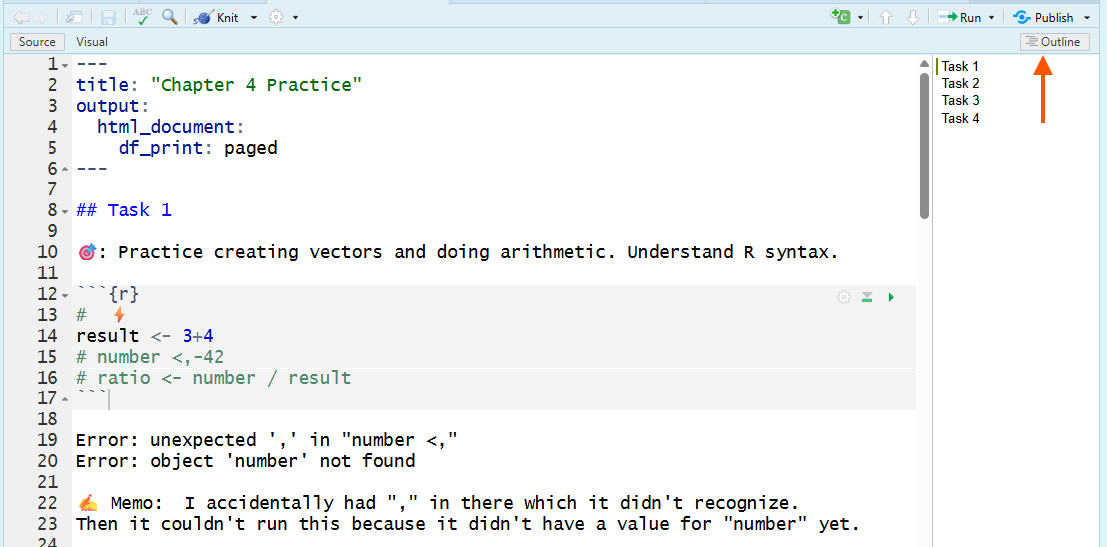
\includegraphics[keepaspectratio]{Memo_Example_heading.png}}

\begin{center}\rule{0.5\linewidth}{0.5pt}\end{center}

This image is a screenshot of an RStudio R Notebook showing a Markdown
section heading (\#\# Task 1) in the editor and the Outline pane on the
right listing ``Task 1--Task 4,'' illustrating that Markdown headings
create a structured outline; the orange arrow points to the Outline
button used to show/hide that heading-based outline.

In this example, the \texttt{\#\#\ Task\ 1} heading creates a main
section heading. The Outline pane on the right lists all headings in the
document, allowing you to navigate quickly between sections.

\subsection{The most common beginner mistake
with}\label{the-most-common-beginner-mistake-with}

``\#'' means two totally different things depending on where you type
it:

\textbf{Outside a code chunk}: \# creates a heading (Markdown
formatting).

\textbf{Inside a code chunk}: \# creates a comment (R ignores it).

\begin{center}\rule{0.5\linewidth}{0.5pt}\end{center}

Now that you have the basics in Markdown, let's practice creating
headings in your R Notebook as you work through R coding exercises.

\chapter{Knit to HTML}\label{knit-to-html}

When you \textbf{Knit} to HTML, RStudio creates a shareable, static
report that includes your formatted headings and text, your code, and
the output produced when the code runs.

This is not the same as ``running a chunk''. Running a chunk uses your
current R session. It can succeed even if you ran things out of order or
if objects already exist in your Environment. Knitting is a full test:
it runs the entire notebook top-to-bottom in a fresh session, then
builds an HTML report.

📏 \textbf{Rule:} Your notebook must create every object it uses in the
notebook itself (not in your Environment).

\subsection{How to Knit}\label{how-to-knit}

RStudio UI varies. Some of you will have a \textbf{Knit button}, others
will use \textbf{Preview menu} dropdown.

Option 1: \textbf{Knit button}

In the Source pane, click the \textbf{Knit button} (it looks like a ball
of yarn with a knitting needle 🧶).

\begin{center}\rule{0.5\linewidth}{0.5pt}\end{center}

\pandocbounded{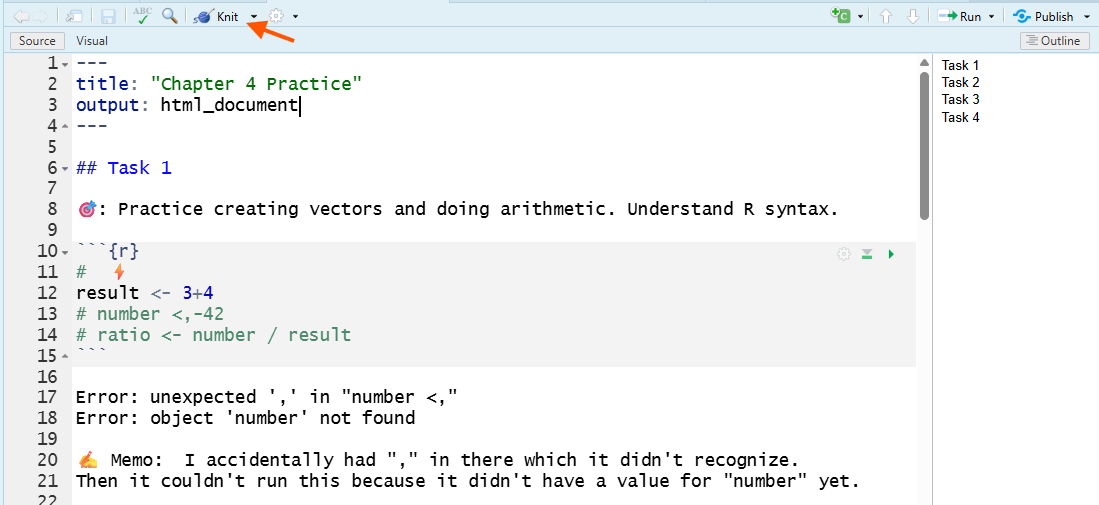
\includegraphics[keepaspectratio]{Memo_Example_knithtml3.png}}

\begin{center}\rule{0.5\linewidth}{0.5pt}\end{center}

This image is a screenshot of RStudio showing the Knit button on the
toolbar (highlighted by an orange arrow), which students can click to
knit the R Notebook into an HTML document when they don't have the
Preview dropdown.

Option 2: \textbf{Preview menu}

In the Source pane, click the the \textbf{Preview menu} drop down button
and select Knit to HTML.

\begin{center}\rule{0.5\linewidth}{0.5pt}\end{center}

\pandocbounded{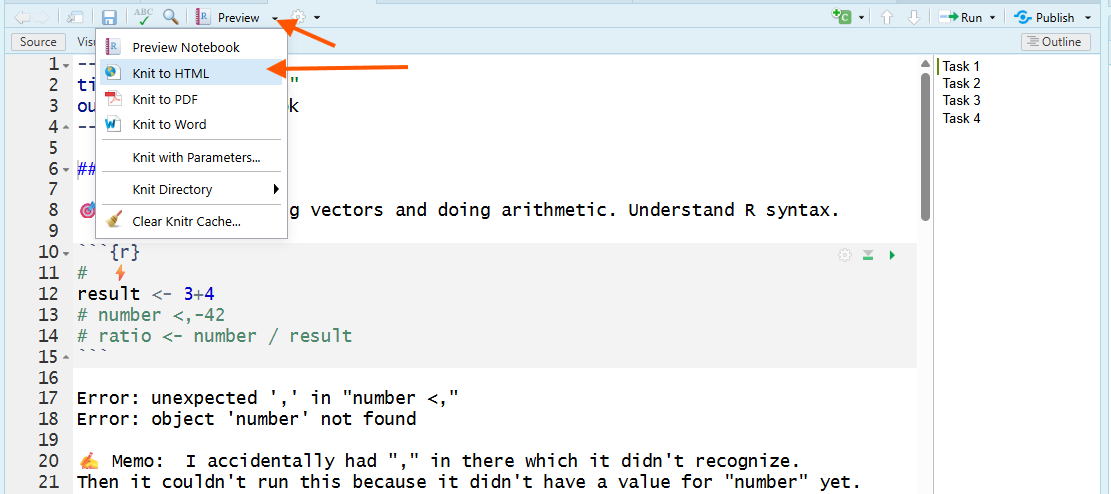
\includegraphics[keepaspectratio]{Memo_Example_knithtml.png}}

\begin{center}\rule{0.5\linewidth}{0.5pt}\end{center}

This image is a screenshot of RStudio with the Preview menu opened;
orange arrows highlight the Preview dropdown button and the Knit to HTML
option, showing how to knit an R Notebook into a shareable HTML document
(not just run a single code chunk).

Below is the result you get after knitting to HTML

\begin{center}\rule{0.5\linewidth}{0.5pt}\end{center}

\pandocbounded{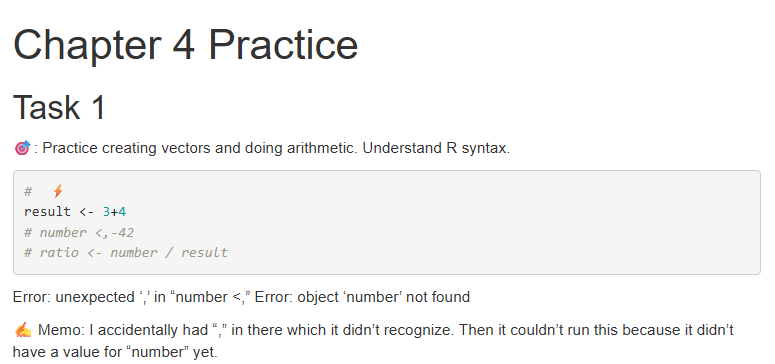
\includegraphics[keepaspectratio]{Memo_Example_knithtml2.png}}

\begin{center}\rule{0.5\linewidth}{0.5pt}\end{center}

This image is a screenshot of the knitted HTML output in a web browser
showing the notebook title (``Chapter 4 Practice''), the first section
heading (``Task 1''), a memo as regular paragraph text, and an R code
chunk with its printed error output, demonstrating what you get after
you Knit to HTML.

When you knit, RStudio automatically does three things:

\begin{enumerate}
\def\labelenumi{\arabic{enumi}.}
\item
  Starts a fresh R session (your Environment does not count).
\item
  Runs your notebook from top to bottom in order.
\item
  Produces an HTML file you can view and share.
\end{enumerate}

This is why knitting is the real test of ``does this notebook work?'' If
it knits, someone else (including future-you) can see the workflow and
results without needing to open RStudio.

\subsection{Submitting the HTML File}\label{submitting-the-html-file}

The HTML file is automatically saved in the same folder as your R
Notebook, with the same name but an \texttt{.html} extension instead of
\texttt{.Rmd}. If you have not yet saved your R Notebook, RStudio will
prompt you to do so before knitting.

Example:

\begin{itemize}
\item
  \texttt{chapter5\_practice.Rmd}
\item
  \texttt{chapter5\_practice.html}
\end{itemize}

💡 \textbf{Tip:} the HTML opens in your browser, but the browser address
is a local file path on your computer. You cannot submit a browser link.

When you open an HTML, it uses your web browser to display a nicely
formatted version of your notebook, including code, output, and memos.
You cannot share the HTML by sharing the web address (URL) in your
browser because it is a local file on your computer.

To submit, 📤 upload the \texttt{.html} file from your course folder
(and follow any Canvas instructions your assignment page provides).

\subsection{Knit Errors}\label{knit-errors}

When you select to knit, the Console pane shows progress messages in the
\textbf{Render tab} as R runs your notebook from top to bottom.

A successful knit has three visible signs:

\begin{enumerate}
\def\labelenumi{\arabic{enumi}.}
\item
  The Render tab shows the process finishing without an error message.
\item
  A browser window opens (or Viewer in File Pane) showing your notebook
  as a formatted web page.
\item
  An \texttt{.html} file appears in the same folder as your
  \texttt{.Rmd} file.
\end{enumerate}

If knitting fails, do not guess. Do this in order:

\begin{enumerate}
\def\labelenumi{\arabic{enumi}.}
\item
  Read the last error message in the \textbf{Render tab}.
\item
  Find the chunk that caused it (the error usually names a chunk or
  shows a line number).
\item
  Fix the first error you see. (Many later errors are just ``domino
  effects.'')
\item
  Knit again.
\end{enumerate}

Common reasons knitting fails:

\begin{itemize}
\item
  You wrote the code out of order, so an object exists in your
  Environment but is not created earlier in the notebook.
\item
  You forgot to include setup code (creating objects, loading packages,
  setting a working directory, etc.).
\item
  A chunk contains an error you didn't notice because you never ran that
  chunk.
\end{itemize}

💡 \textbf{Tip:} When designing your document, knit after any meaningful
formatting or code change. It's the fastest way to catch problems early.
It is easier to determine an error when it is caused by your most recent
editing.

Some errors are tricky. If you get stuck, ask for help.

\chapter{Structuring LLM Prompts}\label{structuring-llm-prompts}

One resource to troubleshooting a knit error, or many other coding
problems, is using a \textbf{Large Language Model} (LLM) like ChatGPT or
boisestate.ai to assist you. However, the quality of the response you
get depends heavily on how you structure your prompt. The same Markdown
you use in your R Notebook can also be used to structure prompts for
LLMs.

\section{Missing Backtick}\label{missing-backtick}

Imagine you don't know that there is a missing backtick at the end of a
code chunk. You try to knit to HTML, but it fails. You ask an LLM to
help you find the error.

Below are three example prompts versions: unstructured (bad), structured
plain text (better), and structured Markdown (best).

\subsection{Unstructured Prompt}\label{unstructured-prompt}

\begin{verbatim}
What do I do? I tried knitting my R notebook and it won’t work. 

|...... | 12% [unnamed-chunk-1]

processing file: Chapter_4_practice.Rmd

Error in parse():
! attempt to use zero-length variable name
Quitting from Chapter_4_practice.Rmd:12-24 [unnamed-chunk-1]
Execution halted
\end{verbatim}

\subsection{Structured Plain Text
Prompt}\label{structured-plain-text-prompt}

\begin{verbatim}
Persona: Act as a R programming tutor.

Task: Help me troubleshoot a knit error in an R Notebook     (`.Rmd`). I am a beginner.

What I did: I clicked Preview > Knit to HTML in RStudio.

What happened: Knitting stopped at 12% and failed.

Error message (*copied from Render tab*):
|...... | 12% [unnamed-chunk-1]
processing file: Chapter_4_practice.Rmd
Error in parse():
! attempt to use zero-length variable name
Quitting from Chapter_4_practice.Rmd:12-24 [unnamed-chunk-1]
Execution halted

Context: The error says it quit from lines 12–24 in     unnamed-chunk-1. I don’t understand what “parse” means.

What I want from you: 1. Explain what this error usually means in beginner-friendly terms. 2. Give me the most likely causes specifically for an R Notebook `.Rmd` file. 3. Give me a checklist of what to look for around lines 12–24 to fix it.
\end{verbatim}

\subsection{Structured Prompt:}\label{structured-prompt}

\begin{verbatim}
# Persona: 

Act as a R programming tutor.

# Task: 

Help me troubleshoot a knit error in an R Notebook (`.Rmd`). 

# What I did: 

In RStudio, I clicked Preview → Knit to HTML.

# What happened: 

Knitting stopped at 12% and failed.

# Error message (copied exactly):
\end{verbatim}

\begin{Shaded}
\begin{Highlighting}[]
\PreprocessorTok{|}\NormalTok{......                                              }\PreprocessorTok{|}\NormalTok{  12\% }\CommentTok{[}\OtherTok{unnamed{-}chunk{-}1}\CommentTok{]}

\NormalTok{processing file: Chapter\_4\_practice.Rmd}

\NormalTok{Error in }\InformationTok{\textasciigrave{}parse()\textasciigrave{}}\NormalTok{:}
\NormalTok{! attempt to use zero{-}length variable name}
\NormalTok{Backtrace:}
\NormalTok{...}
\NormalTok{Quitting from Chapter\_4\_practice.Rmd:12{-}24 }\CommentTok{[}\OtherTok{unnamed{-}chunk{-}1}\CommentTok{]}
\NormalTok{Execution halted}
\end{Highlighting}
\end{Shaded}

\begin{verbatim}
# Context: 

The error says it quit from lines 12–24 in unnamed-chunk-1. I don’t understand what “parse” means.

# What I want from you:

1. Explain what “Error in parse()” means in plain language.

2. Tell me the top 3 most common causes in an `.Rmd` file.

3. Give me a step-by-step fix plan focused on the section lines 12–24.
\end{verbatim}

\begin{center}\rule{0.5\linewidth}{0.5pt}\end{center}

\emph{If you use LLMs to help with R code, always document when and how
you used the tool in your R Notebook. Unless explicitly stated in
assignment instructions, do not ask LLMs to write code for you. Quote
all copy-paste LLM-generated code and write a memo about what you
learned. This maintains academic integrity and helps you understand and
maintain your autonomy as a learner.}

\chapter{Summary}\label{summary}

In Chapter 5, you learned how to use an R Notebook as more than a place
to run code---you learned how to produce a clear, shareable HTML report
that documents your work in a way that another person (or future-you)
can follow. You practiced Markdown basics that make your notebook
readable, including adding a date in the YAML header and using headings
to create an outline. Finally, you learned what it means to generate an
HTML report from your notebook (running everything top-to-bottom in a
fresh session) and how to troubleshoot errors when that process
fails---especially formatting mistakes like broken code chunk
fences---and you practiced writing structured, Markdown-based prompts to
get useful help from an LLM while still documenting your own reasoning
and changes.

\chapter{Chapter Terms}\label{chapter-terms}

\textbf{Backtick}: The ` character (above the Tab key) used for
code-related formatting and quoting. In \textbf{Markdown}, single
backticks mark \emph{inline code} and triple backticks create
\emph{fenced code blocks}; in \textbf{R Markdown}, backticks also mark
\emph{inline R code} (`r \ldots`), including inside YAML fields like
date: ``\,`r Sys.Date()`'', which gets evaluated when you render the
document. In R, backticks can also quote non-syntactic names (e.g.,
names with spaces) so they can be used safely in code.

\textbf{HTML}: A web page file type (\texttt{.html}) written in
\textbf{HyperText Markup Language} that a web browser can open and
display as a formatted document. In this course, Preview/Knit/Render can
create an HTML file (often \texttt{.html} or \texttt{.nb.html}) that
shows your notebook's text, code, and output in the browser; because it
opens from your computer (a local \texttt{file://} path), you can't
submit it by copying the browser address. Upload the HTML file itself.

\textbf{Inline R}: A short R expression written inside backticks with
the prefix \texttt{r} (for example, `r Sys.Date()`) that is evaluated
when you knit/render the document and replaced with its result in the
output. Inline R is used to insert dynamic values (dates, computed
statistics, labels) directly into your narrative text, and it can also
be used in YAML fields like date: ``\,`r Sys.Date()`'' when supported.

\textbf{Knit}: In RStudio, the action that renders an \texttt{.Rmd}
(including an R Notebook) into a finished output file (such as HTML,
PDF, or Word) by running the document's code chunks, inserting their
results, and converting the document to the chosen format. Clicking the
Knit button typically calls \texttt{rmarkdown::render()} in a new, clean
R session, so everything needed to reproduce the result must be created
or loaded in the document itself, and the output file is saved alongside
the \texttt{.Rmd}.

\textbf{Knit Button}: The toolbar button in RStudio that renders an R
Markdown file (\texttt{.Rmd}) into a finished output (e.g., HTML, PDF,
Word) by calling \texttt{rmarkdown::render()} and running the document's
code to generate results. The output file is saved next to the
\texttt{.Rmd} (same base name), and the button's drop-down lets you
choose among available output formats (shortcut: Ctrl/Cmd + Shift + K).

\textbf{Large Language Models (LLMs)}: AI systems trained on massive
collections of text and code to predict and generate language, including
R code and explanations. In an R-learning context, LLMs can help you
brainstorm, interpret error messages, and draft code---but they can also
produce plausible-sounding mistakes, so you must verify outputs,
understand each line you run, and document when and how you used the
tool.

\textbf{Markdown}: A lightweight plain-text formatting syntax used to
write structured documents (headings, lists, links, emphasis, code) in a
way that stays readable as plain text and can be rendered into formats
like HTML on many platforms and tools.

\textbf{Preview Menu}: The drop-down attached to the Preview button in
an R Notebook (\texttt{output:\ html\_notebook}) that lets you generate
a quick notebook preview and choose other render (``knit'') actions
(e.g., HTML/PDF/Word). Preview renders an HTML view using outputs from
chunks you've already run (it does not re-execute code), while knit
options render the full document to the selected output format.

\textbf{Render Tab}: A temporary tab that appears in RStudio's Console
pane when you Knit/Render an R Markdown (\texttt{.Rmd}) or Quarto
(\texttt{.qmd}) document. It shows the rendering log---progress
messages, warnings, and errors---separately from your interactive
Console, and typically includes a Stop control so you can interrupt a
failed or long render.

\textbf{YAML Header}: The metadata section at the top of an R Markdown
or Quarto document, written between \texttt{-\/-\/-} lines, that
controls document settings like the title, author, date, output format
(HTML/PDF/Word), and options for rendering.

\chapter{📝 Practice Space}\label{practice-space}

\textbf{Hack-A\_Prompt}

In this Practice Space, you will write a \textbf{Markdown prompt} that
instructs a Large Language Model (LLM) to generate a specific R code
chunk exactly as shown. The goal is to practice two core research
skills:

\begin{itemize}
\item
  \textbf{Clear specification}: describing code requirements precisely
  (like you would in a methods section)
\item
  \textbf{Reproducibility}: checking that code runs from a clean start
\end{itemize}

\textbf{Before you begin}

\begin{enumerate}
\def\labelenumi{\arabic{enumi}.}
\item
  Created a R Notebook in the Source pane and saved it as
  \texttt{chapter5\_practice.Rmd} in your course folder.
\item
  Start clean: Click the 🧹 \textbf{broom icon} in the Environment pane
  to clear objects.
\item
  Write short memos documenting problems, fixes, and any help you used
  (\textbf{tenacity} + \textbf{transparency}).
\end{enumerate}

\section{Task 1}\label{task-1}

\textbf{Organize your notebook with headings}

🎯 Use Markdown headings to organize your notebook so a reader can
follow your work.

Your notebook must include at least:

\begin{itemize}
\item
  One top-level title heading (Level 1)
\item
  Four section headings (Level 2 or Level 3)
\end{itemize}

Your headings must clearly separate:

\begin{enumerate}
\def\labelenumi{\arabic{enumi}.}
\item
  Your prompt draft
\item
  The LLM output you received
\item
  Your memo comparing output vs target
\item
  Your revision attempt and result
\end{enumerate}

💡 \textbf{Tip:} Headings should describe what's in the section (not
``Section 1'').

\section{Task 2}\label{task-2}

\textbf{Write a prompt that reproduces the target code}

🎯 Write a Markdown-structured prompt that \emph{you think} will makes
an LLM generate a specific R code chunk exactly.

\begin{enumerate}
\def\labelenumi{\arabic{enumi}.}
\item
  Read the target code chunk below. Don't run it yet.
\item
  In your R Notebook, compose a Markdown-structured prompt that you
  think will cause an LLM to output this exact code chunk (same object
  names, same order, same functions).
\end{enumerate}

Rules:

\begin{itemize}
\item
  You cannot copy-paste any part of the target code chunk into your
  prompt.
\item
  You should use the exact names of objects and functions as needed.
\item
  Your prompt must be structured using Markdown headings.
\end{itemize}

\begin{Shaded}
\begin{Highlighting}[]
\CommentTok{\# Target Code Chunk}
\NormalTok{sales\_q1 }\OtherTok{\textless{}{-}} \FunctionTok{c}\NormalTok{(}\DecValTok{120}\NormalTok{, }\DecValTok{135}\NormalTok{, }\DecValTok{150}\NormalTok{, }\DecValTok{160}\NormalTok{)}
\NormalTok{sales\_q2 }\OtherTok{\textless{}{-}} \FunctionTok{c}\NormalTok{(}\DecValTok{125}\NormalTok{, }\DecValTok{130}\NormalTok{, }\DecValTok{155}\NormalTok{, }\DecValTok{170}\NormalTok{)}

\NormalTok{growth }\OtherTok{\textless{}{-}}\NormalTok{ sales\_q2 }\SpecialCharTok{{-}}\NormalTok{ sales\_q1}

\NormalTok{positive\_growth }\OtherTok{\textless{}{-}}\NormalTok{ growth[growth }\SpecialCharTok{\textgreater{}} \DecValTok{0}\NormalTok{]}
\NormalTok{last\_two }\OtherTok{\textless{}{-}}\NormalTok{ sales\_q2[}\FunctionTok{c}\NormalTok{(}\DecValTok{3}\NormalTok{, }\DecValTok{4}\NormalTok{)]}

\FunctionTok{length}\NormalTok{(sales\_q1)}
\FunctionTok{length}\NormalTok{(sales\_q2)}
\FunctionTok{class}\NormalTok{(growth)}
\end{Highlighting}
\end{Shaded}

\section{Task 3}\label{task-3}

\textbf{Test your prompt and document what happened}

🎯 Test your prompt in an LLM \emph{(recommend boisestate.ai).}

\begin{enumerate}
\def\labelenumi{\arabic{enumi}.}
\item
  Paste your prompt into the LLM chat box and submit it.
\item
  Place the LLM's output an a code chunk in your notebook and run it.
\item
  Write a memo (4--8 sentences) that includes:
\end{enumerate}

\begin{itemize}
\item
  What matched the target exactly
\item
  What did not match
\item
  What you changed (or will change) in the prompt to fix it
\item
  State the name of the LLM that you used.
\end{itemize}

\section{Task 4}\label{task-4}

\textbf{Revise your prompt and retest}

Could you improve your prompt?

🎯 Revise your prompt until you get the \textbf{exact} target code
chunk.

💡 \textbf{Tip:} Review and use Chapter 4's \textbf{Chapter Terms}.

\begin{itemize}
\item
  Include at least one revised prompt attempt
\item
  Include the revised LLM output
\item
  Include a short memo explaining what you changed and why
\end{itemize}

\section{Task 5}\label{task-5}

🎯 \textbf{Step 1: Sweep your Environment (start clean).}\\
Click the 🧹 \textbf{broom icon} in the Environment pane to clear
objects.

🎯 \textbf{Step 2: Run everything top-to-bottom.}\\
Use \textbf{Run → Run All} to execute every chunk in order.

🎯 \textbf{Step 3: Save and submit.}\\
After your notebook runs without errors, save your notebook
(\texttt{.Rmd}) and knit to HTML (\texttt{.HTML}) for submission to
Canvas, as directed.

If you have any issues knitting, document the error message, your
troubleshooting steps, and any help you used in your notebook.

\bibliography{references.bib}

\end{document}
